\newpage
\section{Auswertung}

In diesem Abschnitt wird der Versuch ausgewertet.

\subsection{Vorbereitungsaufgabe}
Als Vorbereitungsaufgabe für den Versuch wurden die Dopplerwinkel $\alpha$ zu den Prismenwinkel $\theta = 15° , 30°$ und $60°$.

\begin{table}
    \centering
    \caption{Prismenwinkel zu Dopplerwinkel}
    \begin{tabular}{c c}
        \toprule
        {$\theta$} & {$\alpha$}  \\
        \midrule
        15° & 80.06411625951776°  \\
        30° & 70.52877936550931°  \\
        60° & 54.735610317245346°  \\
        \bottomrule
    \end{tabular}
    \label{tab:vor}
\end{table}

\subsection{Bestimmung der Strömungsgeschwindigkeit}

Die aufgenommen Messwerte bei den unterschiedlichen Rohr Innendurchmessern $d$ werden in die Tabelle (\ref{tab:a}) eingetragen.

\begin{table}
    \centering
    \caption{Messergebnisse der Dopplerverschiebung}
    \begin{tabular}{c | c c c c}
        \toprule
        {$d \, \si{\milli\meter} $} & {$Flussgeschwindigkeit \, \si{\liter\per\minute}$} & {$Dopplerwinkel bei 15°$} & {$Dopplerwinkel bei 30°$} & {$Dopplerwinkel bei 60°$} \\
        \midrule
    7 &    2     &      55    &      195   &      378    \\
     &    3      &     146    &     342    &     647   \\
     &    4      &     244    &     525    &     989   \\
     &    5      &     354    &     732    &     1385   \\
     &    6      &     452    &     964    &     1843   \\
     &    7.5    &     647    &     1367   &     2515   \\
    \midrule 
    10 &    2     &      -49  &       85     &     -122 \\
     &    3       &    -73    &     134      &   -220 \\
     &    4       &    -110   &     208      &   -342 \\
     &    5       &    -146   &     305      &   -464 \\
     &    6       &    -183   &     403      &   -647 \\
     &    7.5     &    -256   &     598      &   -879 \\
    \midrule 
    16 &    2      &     49  &        49   &       61 \\
     &    3        &   61    &      73     &     122 \\
     &    4        &   73    &      110    &     183 \\
     &    5        &   98    &      134    &     256 \\
     &    6        &   110   &      171    &     342 \\
     &    7.5      &   171   &      256    &     500 \\
        \bottomrule
    \end{tabular}
    \label{tab:a}
\end{table}

\noindent
Mithilfe der Formel (\ref{equ:Geschw}) und der verwendeten Ultraschallsonde mit $\nu_0 = 2 \si{\mega\hertz} $ lässt sich die Strömungsgeschwindigkeit $\nu$, sowie dem Winkel $\alpha$ bestimmen. Diese werden in die Tabelle (\ref{tab:b}) eingetragen.

\begin{equation}
    \label{equ:Geschw}
    v = \frac{\increment \nu \cdot c}{2\nu \cdot cos(\alpha)}
\end{equation}


\begin{table}
    \centering
    \caption{Berechnete Flussgeschwindigkeit in Abhängigkeit des Winkels}
    \begin{tabular}{c | c c c c}
        \toprule
        {$d \, in \, \si{\milli\meter} $} & {$Flussgeschwindigkeit \, in \, \si{\liter\per\minute}$} & {$\nu \, bei 15° \, in \,in \, \si{\meter\per\second}$} & {$\nu \, bei 30° \, in \, \si{\meter\per\second}$} & {$\nu \, bei 60° \, in \, \si{\meter\per\second}$} \\
        \midrule
    7mm &    2     &      0.14343999    &      0.26325   &      0.29462184 \\
     &    3      &     0.38076796    &     0.4617    &     0.50428659 \\
     &    4      &     0.63635193    &     0.70875    &     0.77084921 \\
     &    5      &     0.9232319    &     0.9882    &     1.07950067 \\
     &    6      &     1.17881588    &     1.3014    &     1.43647634 \\
     &    7.5    &     1.68737583    &     1.84545   &     1.9602485 \\
    \midrule
    10 &    2     &      -0.12779199  &       0.11475     &     -0.09508959  \\
     &    3       &    -0.19038398    &     0.1809      &    -0.17147303  \\
     &    4       &    -0.28687997   &     0.2808      &   -0.26656262  \\
     &    5       &    -0.38076796   &     0.41175      &   -0.36165221  \\
     &    6       &    -0.47726395   &     0.54405      &   -0.50428659  \\
     &    7.5     &    -0.66764793   &     0.8073      &   -0.6851127  \\
    \midrule
    16 &    2      &     0.12779199  &        0.06615   &       0.04754479  \\
     &    3        &   0.15908798    &      0.09855     &     0.09508959 \\
     &    4        &   0.19038398    &      0.1485    &     0.14263438 \\
     &    5        &   0.25558397    &      0.1809    &     0.19953225 \\
     &    6        &   0.28687997   &      0.23085    &     0.26656262 \\
     &    7.5      &   0.44596795   &      0.3456    &     0.38971143 \\

        \bottomrule
    \end{tabular}
    \label{tab:b}
\end{table}

\noindent
Die foglenden Grafiken zeigen $\frac{\increment \nu}{cos(\alpha)}$ in Abhängigkeit von der Strömungsgeschwindigkeit, für alle drei Rohr Innendurchmesser.

\begin{figure}
    \centering
    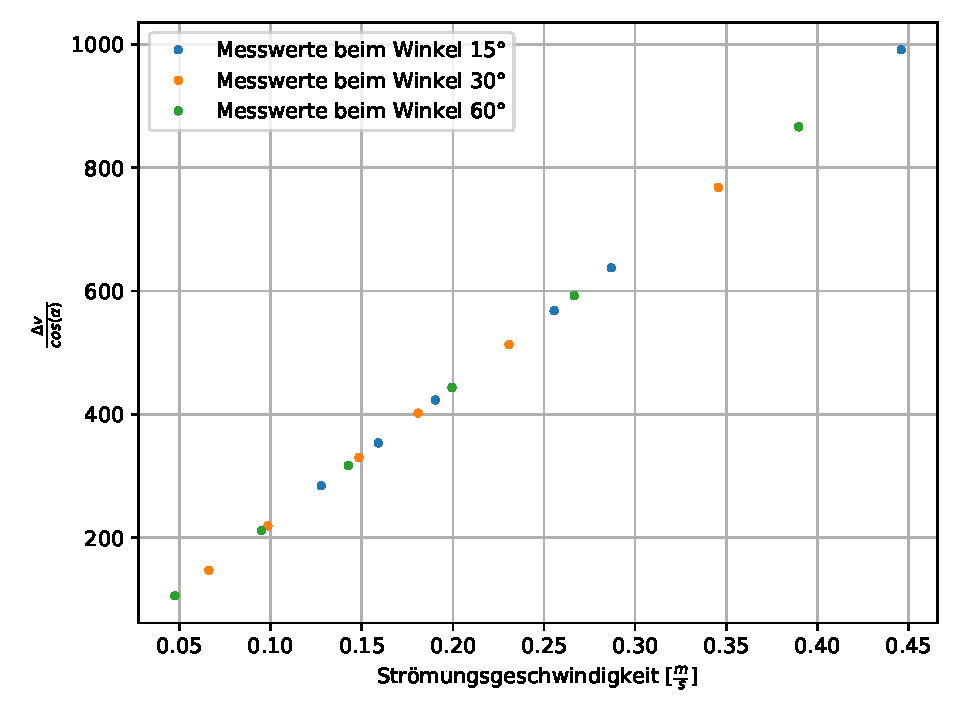
\includegraphics{7mm.pdf}
    \caption{Verhältnis der Frequenzverschiebung zum Dopplerwinkel abhängig von der Strömungsgeschwindigkeit.}
    \label{fig:KeineAhnung}
\end{figure}

\begin{figure}
    \centering
    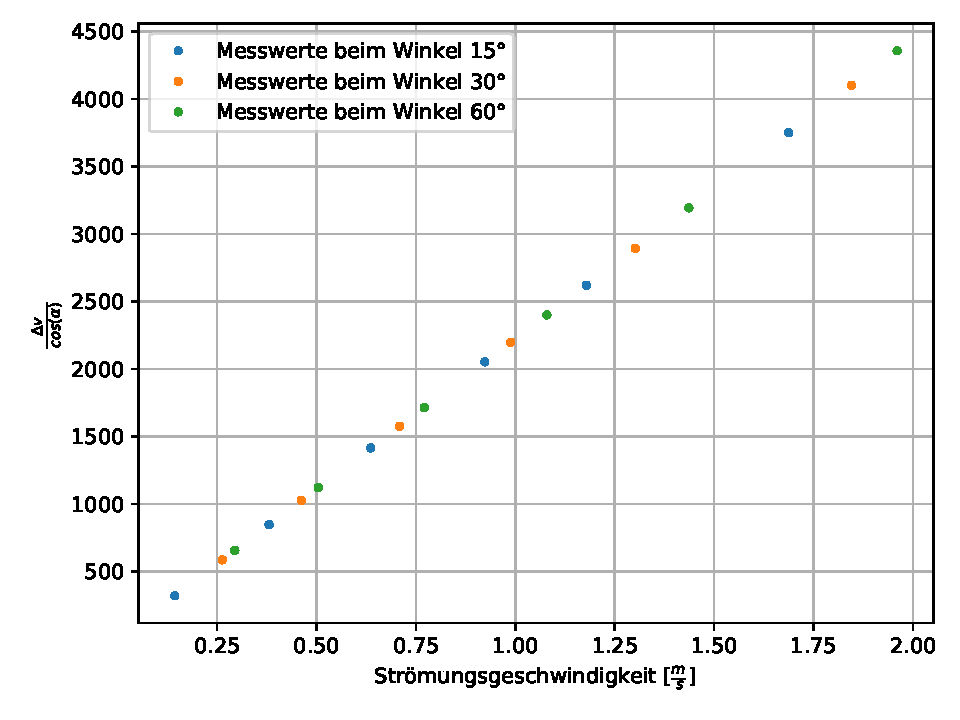
\includegraphics{10mm.pdf}
    \caption{Verhältnis der Frequenzverschiebung zum Dopplerwinkel abhängig von der Strömungsgeschwindigkeit.}
    \label{fig:KeineAhnung}
\end{figure}
\begin{figure}
    \centering
    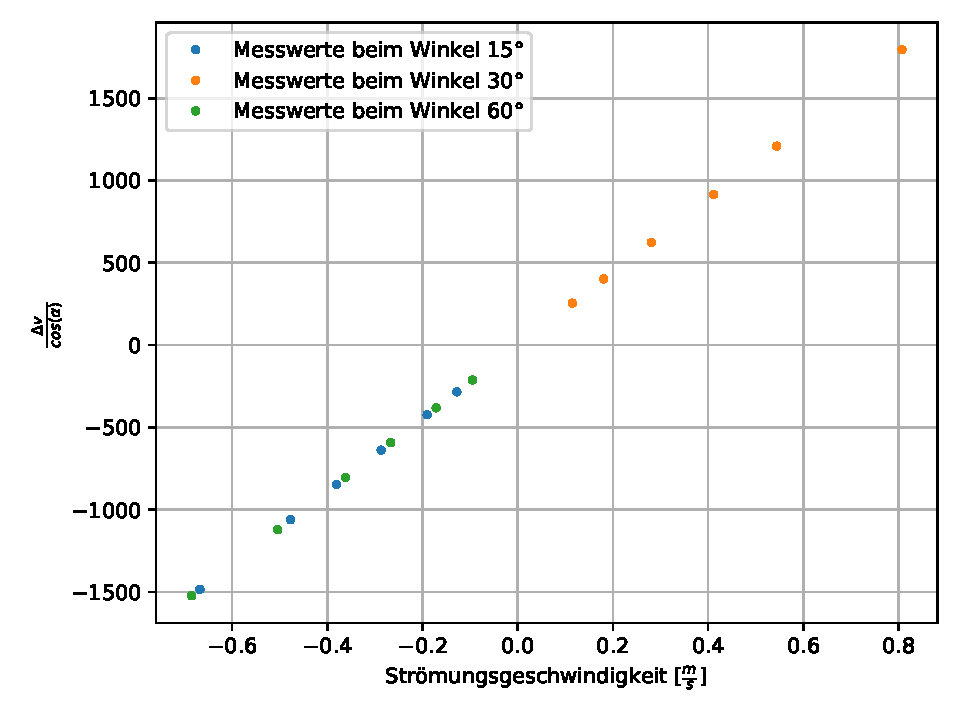
\includegraphics{16mm.pdf}
    \caption{Verhältnis der Frequenzverschiebung zum Dopplerwinkel abhängig von der Strömungsgeschwindigkeit.}
    \label{fig:KeineAhnung}
\end{figure}